\documentclass[12pt,a4paper]{report}

\usepackage[a4paper,left=40mm,right=25mm,top=25mm,bottom=40mm]{geometry}
\usepackage{mathptmx}
\usepackage{amsmath}
\usepackage{setspace}
\usepackage{graphicx}
\usepackage{booktabs}
\usepackage{longtable}
\usepackage{array}
\usepackage{float}
\usepackage{caption}
\usepackage[hidelinks]{hyperref}
\usepackage{url}
\Urlmuskip=0mu plus 1mu
\setlength{\emergencystretch}{2em}
\sloppy

\onehalfspacing
\setcounter{secnumdepth}{3}
\setcounter{tocdepth}{3}
\graphicspath{{../../../latex/}}

% Template-aligned heading styles without extra packages
\makeatletter
\def\@makechapterhead#1{%
  \vspace*{20pt}%
  {\parindent \z@ \raggedright \normalfont
    \ifnum \c@secnumdepth >\m@ne
      \bfseries\fontsize{14pt}{18pt}\selectfont \@chapapp\ \thechapter
      \par\nobreak
      \vskip 10pt
    \fi
    \interlinepenalty\@M
    \bfseries\fontsize{14pt}{18pt}\selectfont \MakeUppercase{#1}\par\nobreak
    \vskip 20pt
  }}
\def\@makeschapterhead#1{%
  \vspace*{20pt}%
  {\parindent \z@ \raggedright
    \normalfont
    \interlinepenalty\@M
    \bfseries\fontsize{14pt}{18pt}\selectfont \MakeUppercase{#1}\par\nobreak
    \vskip 20pt
  }}
\renewcommand\section{\@startsection{section}{1}{\z@}%
  {-3.5ex \@plus -1ex \@minus -.2ex}%
  {2.3ex \@plus.2ex}%
  {\normalfont\bfseries\fontsize{12pt}{16pt}\selectfont}}
\renewcommand\subsection{\@startsection{subsection}{2}{\z@}%
  {-3.25ex\@plus -1ex \@minus -.2ex}%
  {1.5ex \@plus .2ex}%
  {\normalfont\bfseries\fontsize{12pt}{16pt}\selectfont}}
\makeatother

\newcommand{\projecttitle}{NEXAR: INTELLIGENT QUANTUM-CLASSICAL WORKLOAD ROUTING PLATFORM}
\newcommand{\degree}{B.Sc. (Hons) Degree in Information Technology Specializing in Software Engineering}
\newcommand{\department}{Department of Information Technology}
\newcommand{\university}{Sri Lanka Institute of Information Technology}
\newcommand{\submissionmonth}{April 2026}
\newcommand{\country}{Sri Lanka}
\newcommand{\titlepagedeclare}{Dissertation submitted in partial fulfilment of the requirements for}

\begin{document}
\hypersetup{pageanchor=false}

% Formal title page
\begin{titlepage}
\centering
\vspace*{1.0cm}
{\bfseries\fontsize{16pt}{20pt}\selectfont \projecttitle\par}
\vspace{2.0cm}
{\fontsize{14pt}{18pt}\selectfont
Siriwardhana A H L T S (IT22094568)\\
Prasad H G A T (IT22056870)\\
Jayasinghe Y L (IT22103840)\\
Hettiarachchi S R (IT22128386)\par}
\vspace{2.0cm}
{\fontsize{12pt}{18pt}\selectfont
\titlepagedeclare\\
\degree\par}
\vspace{2.0cm}
{\fontsize{14pt}{18pt}\selectfont
\department\par}
\vspace{0.6cm}
{\fontsize{14pt}{18pt}\selectfont
\university\\
\country\\
\submissionmonth\par}
\end{titlepage}

\pagenumbering{roman}
\hypersetup{pageanchor=true}

\chapter*{DECLARATION}
\addcontentsline{toc}{chapter}{Declaration}
We declare that this dissertation is our own work and does not incorporate, without acknowledgement, any material previously submitted for a degree or diploma in any university or institute of higher learning. To the best of our knowledge and belief, it does not contain any material previously published or written by another person except where acknowledgement is made in the text.

We hereby grant Sri Lanka Institute of Information Technology the non-exclusive right to reproduce and distribute this dissertation, in whole or in part, in print, electronic, or other media. We retain the right to use this content in whole or part in future works such as articles or books.

\vspace{1cm}
\begin{longtable}{p{0.42\textwidth}p{0.22\textwidth}p{0.22\textwidth}}
\toprule
\textbf{Name} & \textbf{Signature} & \textbf{Date} \\
\midrule
Siriwardhana A H L T S & & \\
\addlinespace[1.2cm]
Prasad H G A T & & \\
\addlinespace[1.2cm]
Jayasinghe Y L & & \\
\addlinespace[1.2cm]
Hettiarachchi S R & & \\
\bottomrule
\end{longtable}

\vspace{0.5cm}
The above candidates have carried out research for the undergraduate dissertation under our supervision.

\vspace{1cm}
\begin{longtable}{p{0.42\textwidth}p{0.22\textwidth}p{0.22\textwidth}}
\toprule
\textbf{Supervisor} & \textbf{Signature} & \textbf{Date} \\
\midrule
Prof. Nuwan Kodagoda & & \\
\addlinespace[1.2cm]
Dr. Kapila Dissanayake & & \\
\bottomrule
\end{longtable}

\chapter*{ACKNOWLEDGEMENT}
\addcontentsline{toc}{chapter}{Acknowledgement}
The Nexar research team wishes to express sincere gratitude to Prof. Nuwan Kodagoda and Dr. Kapila Dissanayake for their guidance, feedback, and supervision throughout the design, implementation, and evaluation of this research. Their direction helped the team frame the work not only as a software engineering project, but also as a research contribution to hybrid quantum-classical computing.

We also thank the Department of Information Technology and Sri Lanka Institute of Information Technology for providing the academic environment, infrastructure, and research support required to complete a project of this scope. The open-source quantum computing and software engineering communities, especially the contributors to Qiskit, FastAPI, React, HuggingFace Transformers, scikit-learn, XGBoost, Redis, Terraform, and Google Cloud Platform, provided the technical foundation on which the implementation was built.

Finally, we thank our families, friends, and peers for their patience and encouragement during the development and documentation of Nexar.

\chapter*{ABSTRACT}
\addcontentsline{toc}{chapter}{Abstract}
The Noisy Intermediate-Scale Quantum (NISQ) era has made quantum hardware accessible through cloud platforms, yet practical adoption remains limited by the difficulty of deciding when a workload should execute on quantum hardware, a quantum simulator, or classical infrastructure. Nexar addresses this problem through an intelligent quantum-classical workload routing platform that accepts source code, analyses its computational and quantum characteristics, recommends the most suitable execution target, converts selected classical algorithms into quantum implementations, and dispatches workloads through a provider-agnostic execution layer.

The system is implemented as a six-service microservice platform consisting of a React frontend, an Express API Gateway, a Code Analysis Engine, an AI Code Converter, a Decision Engine, and a Hardware Abstraction Layer. The Code Analysis Engine detects Python, Qiskit, Cirq, Q\#, and OpenQASM code with 98.52\% language-classification accuracy and performs algorithm and complexity analysis. The AI Code Converter fine-tunes CodeT5 for classical-to-Qiskit translation, achieving a 98.7\% valid Qiskit generation rate on a held-out evaluation set. The Decision Engine combines machine learning, physics-aware rules, and cost analysis through a two-stage routing pipeline. Against 100 benchmark workloads and two independently defined routing oracles, Nexar achieves 0.810--0.860 accuracy, F1(Q) of 0.457--0.500, and perfect Quantum-class recall under the hardware-viability oracle. The Hardware Abstraction Layer validates provider-agnostic execution through IBM Quantum integration, job lifecycle management, calibration-aware device listing, sandboxed Python execution, and real-hardware tests on 27 circuits.

The results show that Nexar provides a practical foundation for automated hybrid quantum-classical orchestration, while also identifying limitations in synthetic-to-real model transfer, provider coverage, and NISQ hardware fidelity.

\textbf{Keywords:} quantum-classical routing, NISQ, code analysis, CodeT5, decision engine, hardware abstraction layer, Qiskit, workload orchestration.

\tableofcontents
\listoftables
\listoffigures

\chapter*{LIST OF ABBREVIATIONS}
\addcontentsline{toc}{chapter}{List of Abbreviations}
\begin{longtable}{p{0.18\textwidth}p{0.72\textwidth}}
API & Application Programming Interface \\
AST & Abstract Syntax Tree \\
AWS & Amazon Web Services \\
CAE & Code Analysis Engine \\
CI/CD & Continuous Integration / Continuous Deployment \\
GCP & Google Cloud Platform \\
HAL & Hardware Abstraction Layer \\
IBM & International Business Machines Corporation \\
IR & Intermediate Representation \\
JWT & JSON Web Token \\
ML & Machine Learning \\
NISQ & Noisy Intermediate-Scale Quantum \\
QAOA & Quantum Approximate Optimization Algorithm \\
QASM & Quantum Assembly Language \\
QCCR & Quantum-Classical Code Router \\
QFT & Quantum Fourier Transform \\
QPE & Quantum Phase Estimation \\
QPU & Quantum Processing Unit \\
REST & Representational State Transfer \\
ROI & Return on Investment \\
VQE & Variational Quantum Eigensolver \\
\end{longtable}

\clearpage
\pagenumbering{arabic}

\chapter{INTRODUCTION}

\section{Background and Literature Survey}
Quantum computing uses superposition, entanglement, and interference to process information in ways that differ fundamentally from classical computation. Algorithms such as Shor's factorization algorithm and Grover's search algorithm established that specific problem classes can receive theoretical speedups on quantum hardware. However, the present NISQ generation of quantum processors remains constrained by limited qubit counts, gate noise, decoherence, queue delays, and high execution cost. These constraints mean that quantum execution is not automatically beneficial even when a quantum algorithm exists.

The practical engineering problem is therefore a workload-placement problem. Given a piece of source code, the system must identify the programming language and algorithm family, estimate classical and quantum resource requirements, determine whether quantum execution is technically feasible, compare the expected cost and runtime of each execution path, and submit the workload to an appropriate backend. Existing platforms such as Qiskit Runtime, Amazon Braket, and Azure Quantum provide access to quantum devices, but generally assume that the user has already decided to execute quantum code. Existing hardware-selection systems operate on quantum workflows that are already classified as quantum. Nexar is designed to operate one level earlier: it starts from user-submitted source code and automates analysis, routing, optional conversion, and execution.

\section{Research Gap}
The reviewed literature and project investigations show five major gaps. First, there is no unified platform that accepts arbitrary source code and performs code analysis, quantum suitability estimation, routing, conversion, and execution as one workflow. Second, existing code-analysis tools are usually framework-specific and do not provide consistent analysis across Python, Qiskit, Cirq, Q\#, and OpenQASM. Third, classical-to-quantum conversion is still limited, with most available tools focusing on low-level circuit synthesis rather than high-level algorithmic transformation. Fourth, routing decisions often ignore the economics of cloud quantum computing, even though QPU time is expensive relative to classical compute. Fifth, multi-provider quantum execution requires substantial provider-specific integration, making it difficult for routing systems to dispatch workloads across IBM Quantum, Amazon Braket, Azure Quantum, and classical backends through a single interface.

\section{Research Problem}
The central research problem is:

\begin{quote}
How can an integrated software platform automatically analyse user-submitted source code, determine its suitability for quantum or classical execution, optionally convert supported classical algorithms into quantum code, and dispatch the workload to the most suitable backend while considering technical feasibility, cost, runtime, and hardware availability?
\end{quote}

This problem decomposes into four component problems. The Code Analysis Engine must identify source-code language, algorithm type, classical complexity, and quantum circuit characteristics. The AI Code Converter must identify supported classical algorithms and generate correct Qiskit implementations. The Decision Engine must combine ML prediction, deterministic safety rules, and cost analysis into a defensible routing recommendation. The Hardware Abstraction Layer must execute jobs through a unified provider interface while managing job lifecycle, status, results, and device metadata.

\section{Research Objectives}
\subsection{Main Objective}
The main objective of this research is to design, implement, and evaluate Nexar, an intelligent quantum-classical workload routing platform that enables non-specialist users and developers to submit code and receive automated execution recommendations across quantum and classical backends.

\subsection{Specific Objectives}
\begin{enumerate}
\item Develop a multi-language Code Analysis Engine that detects programming language, computes classical and quantum metrics, and classifies algorithm families.
\item Develop an AI Code Converter that translates a defined set of classical Python algorithm patterns into executable Qiskit implementations.
\item Develop a Decision Engine that combines machine learning, physics-aware rule validation, and cost analysis for quantum-classical routing.
\item Develop a provider-agnostic Hardware Abstraction Layer that supports quantum and classical job submission, device discovery, status tracking, and result retrieval.
\item Integrate all components through a React frontend and Express API Gateway into a deployable microservice platform.
\item Evaluate the platform using synthetic held-out tests, a 100-workload benchmark, cost analysis, pipeline latency measurements, and real IBM Quantum hardware validation.
\end{enumerate}

\section{Scope and Delimitations}
This dissertation focuses on practical NISQ-era workload routing rather than fault-tolerant quantum computing. The scope includes code ingestion, analysis, routing, optional conversion, and backend execution orchestration. The system covers four core technical component domains: code intelligence, conversion intelligence, decision intelligence, and execution abstraction.

The study deliberately limits conversion to a defined set of algorithm mappings and does not claim arbitrary classical-program conversion. The provider abstraction is implemented across multiple provider interfaces, but full production-level execution integration is currently validated only on IBM Quantum. The benchmarking scope emphasizes representative and diverse workloads, yet still reflects a bounded sample (100 workloads) suitable for research-grade evaluation rather than full enterprise production benchmarking.

\section{Research Significance}
The significance of this work is both technical and practical. Technically, the project demonstrates an end-to-end architecture that integrates analysis, machine learning, deterministic constraints, cost-awareness, and provider abstraction in one deployable system. Practically, it reduces adoption friction for organizations and students that can write classical code but cannot manually decide quantum viability for each workload.

This work also contributes methodological clarity for hybrid quantum-classical routing studies. It separates algorithmic-advantage reasoning from hardware-viability reasoning through dual-oracle evaluation, showing that routing quality depends on which reality model is being optimized. This distinction is critical in NISQ-era research, where theoretical speedup and practical execution success are often misaligned.

\section{Organisation of the Dissertation}
The remainder of this dissertation is organized as follows. Chapter 2 details the methodology, including system architecture, component-level implementation strategy, deployment, commercialization perspective, and test strategy. Chapter 3 presents quantitative and qualitative results, including model metrics, routing behaviour, hardware validation, and critical discussion. Chapter 4 concludes the study, summarises contributions, and provides future work directions. Appendices provide implementation artefacts, endpoint contracts, testing matrices, and operational references supporting reproducibility and auditability.

\chapter{METHODOLOGY}

\section{Overall System Architecture}
Nexar is structured as a microservices monorepo with six independently deployable services. The frontend provides the user interface for code submission and result visualisation. The API Gateway provides authentication, request routing, logging, and service coordination. The Code Analysis Engine, AI Code Converter, Decision Engine, and Hardware Abstraction Layer are implemented as FastAPI services.

\begin{figure}[H]
\centering
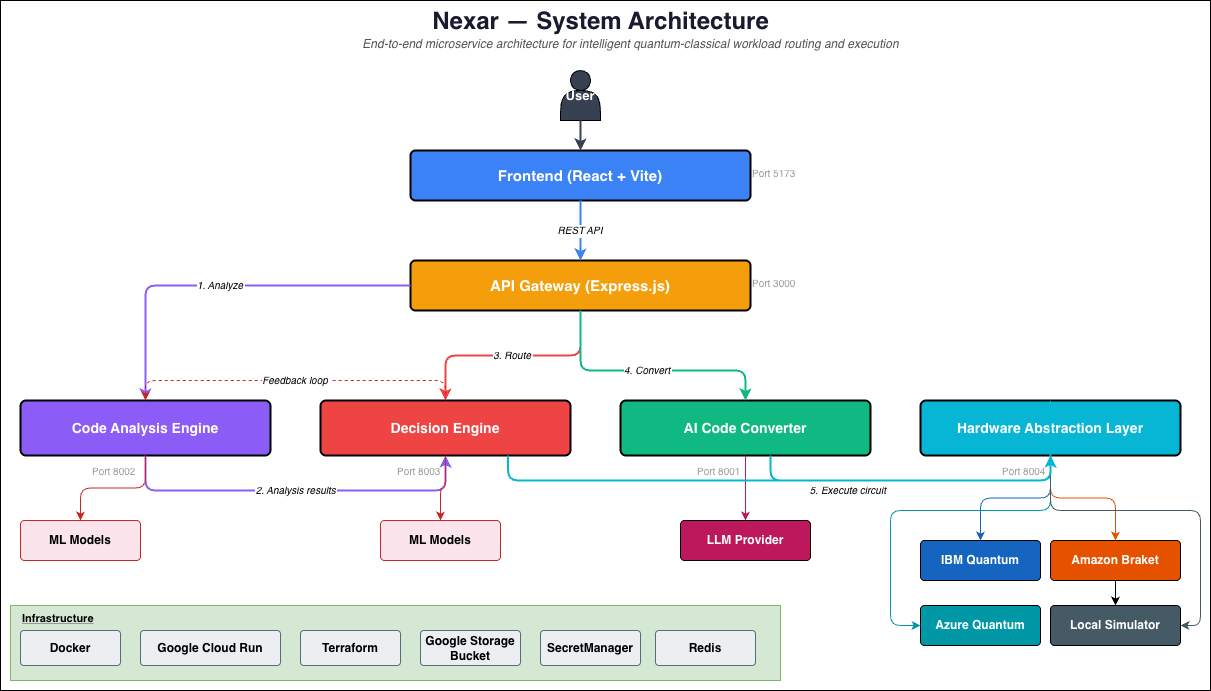
\includegraphics[width=0.95\textwidth]{system-architecture.png}
\caption{Nexar system architecture}
\label{fig:system-architecture}
\end{figure}

The request flow begins when a user submits code through the frontend. The API Gateway validates the request and forwards the code to the Code Analysis Engine. The analysis result is passed to the Decision Engine, which recommends classical execution, quantum simulation, real quantum execution, or rejection. If quantum execution is selected and the input is classical code in a supported algorithm category, the AI Code Converter generates Qiskit code. The Hardware Abstraction Layer then submits the workload to the selected backend and returns job status and results through the API Gateway.

\subsection{Service Boundaries and Responsibilities}
The architecture follows explicit service boundaries to preserve maintainability and independent deployability. The frontend owns interaction design and result presentation, while the API Gateway owns ingress policy and inter-service routing. The Code Analysis Engine owns semantic and structural feature extraction. The AI Code Converter owns transformation logic and conversion confidence. The Decision Engine owns recommendation generation and rationale scoring. The Hardware Abstraction Layer owns execution dispatch and job lifecycle management.

This separation enables each service to evolve independently. For example, model retraining in the Code Analysis Engine can occur without changing execution APIs. Similarly, provider updates in the HAL do not require changes to decision logic as long as provider contracts remain stable.

\subsection{Cross-Service Data Contracts}
All inter-service communication uses JSON contracts over HTTP. The analysis contract includes language predictions, complexity features, algorithm signals, and quantum metrics. The decision contract adds routing labels, confidence, and cost summaries. The execution contract includes provider target, backend device, compiled payload, and run options such as shots and priority. Response contracts include trace identifiers, status transitions, execution metadata, and result payloads.

To reduce integration ambiguity, each service validates incoming data using schema-driven validation (Pydantic for Python services; TypeScript type checks for Node services). Invalid payloads are rejected with explicit error bodies to maintain deterministic behaviour across pipeline failures.

\subsection{Operational Assumptions}
The current design assumes cloud-accessible execution backends, stable API Gateway availability, and model artifacts preloaded or downloadable at service startup. It also assumes that most user workloads are either classical or low-to-mid scale quantum programs, with only a minority falling into large-circuit physical necessity routing paths. This assumption influenced queue strategy and timeout defaults.

\section{Technology Stack}
\begin{table}[H]
\centering
\caption{Core technology stack}
\begin{tabular}{p{0.28\textwidth}p{0.58\textwidth}}
\toprule
\textbf{Layer} & \textbf{Technologies} \\
\midrule
Frontend & React 18, TypeScript, Vite, Tailwind CSS \\
API Gateway & Express 5, TypeScript, JWT authentication \\
Python services & FastAPI, Pydantic, Uvicorn \\
Machine learning & CodeBERT, CodeT5, scikit-learn, XGBoost, HuggingFace Transformers \\
Quantum frameworks & Qiskit, Qiskit Aer, Qiskit Runtime, OpenQASM support \\
Persistence and messaging & Redis, Google Cloud Pub/Sub \\
Deployment & Docker, Google Cloud Run, Artifact Registry, Terraform, GitHub Actions \\
\bottomrule
\end{tabular}
\end{table}

\subsection{Rationale for Technology Choices}
FastAPI was selected for Python microservices due to strong schema validation, automatic OpenAPI generation, and low-friction service composition. React with TypeScript was selected for frontend reliability and maintainability under rapid iteration. The API Gateway uses Express and TypeScript to align with existing team skillsets and simplify JWT middleware integration.

scikit-learn and XGBoost were selected for interpretable baseline and ensemble-friendly ML behaviour under tabular feature regimes. HuggingFace transformer models were selected for code semantics tasks where token-level context is important. Docker and Cloud Run were selected for reproducible deployments, managed scaling, and environment parity across developer and production targets.

\subsection{Infrastructure and Environment Management}
Configuration follows environment-variable driven service configuration. Each service has a dedicated \texttt{.env.example} and startup contract. Secrets are expected from secure stores in deployed environments. Build artefacts are containerized per service and published to Artifact Registry, while Terraform tracks cloud resources declaratively.

This approach enforces repeatable environment provisioning and reduces hidden environment drift. The same service image can be promoted across stages by configuration injection rather than source modification.

\section{Code Analysis Engine}
The Code Analysis Engine transforms raw source code into a structured analysis report consumed by the Decision Engine. Its pipeline combines language detection, classical static analysis, quantum circuit analysis, and algorithm classification.

\begin{figure}[H]
\centering
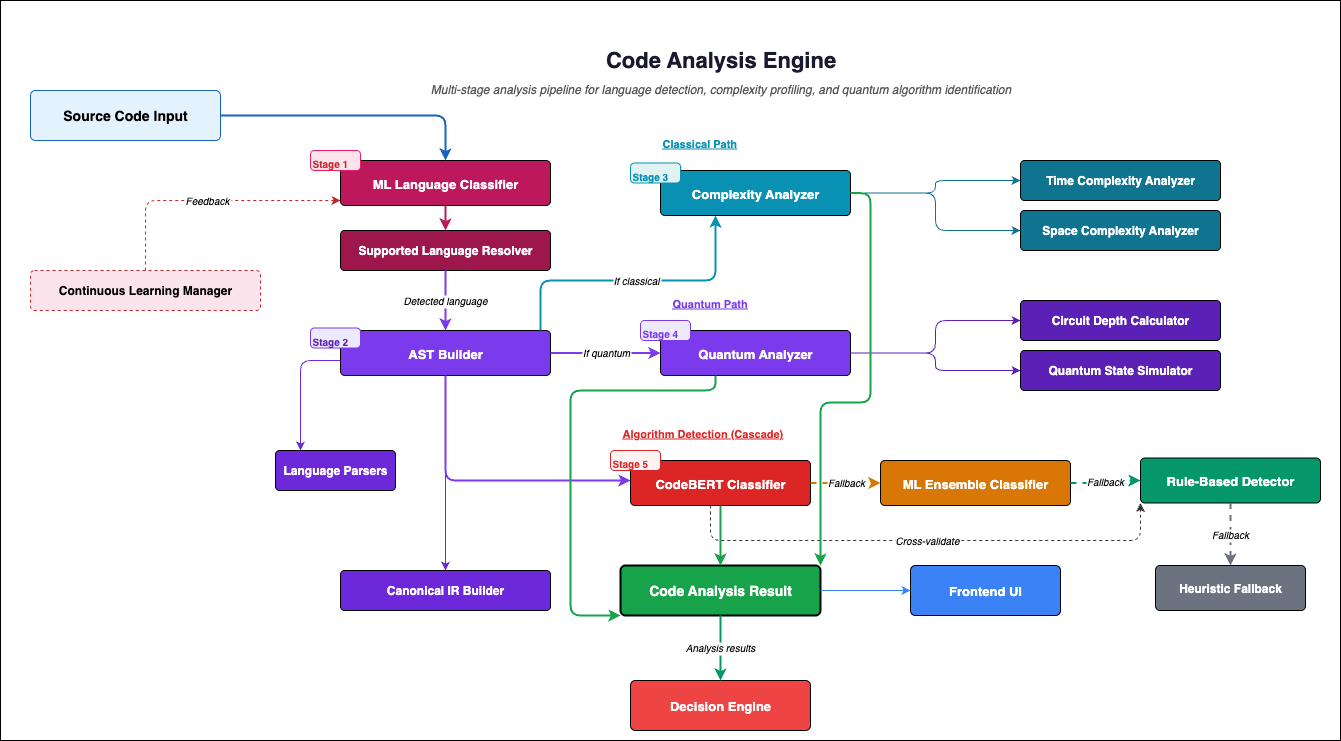
\includegraphics[width=0.85\textwidth]{code-analysis.png}
\caption{Code Analysis Engine pipeline}
\label{fig:code-analysis}
\end{figure}

\subsection{Language Classification}
The language classifier supports Python, Qiskit, Cirq, Q\#, and OpenQASM. It uses a soft-voting ensemble combining CodeBERT, XGBoost, Random Forest, and Gradient Boosting. The ensemble was trained and evaluated on labelled samples covering the supported languages and frameworks. Qiskit and Cirq are intentionally treated as distinct classes even though both are Python-hosted frameworks, because downstream quantum analysis requires framework-specific parsing.

\subsection{Dataset Construction and Curation}
Language and algorithm datasets were assembled from curated code samples, synthetic augmentations, and benchmark-inspired snippets. For language classification, class balance was actively monitored to avoid overwhelming minority classes such as Q\#. For algorithm classification, representative canonical implementations and stylistic variants were included to reduce overfitting to one coding style.

Data curation included deduplication, structural sanity checks, and split-level leakage checks. Training and evaluation splits were separated by sample identity to prevent memorization effects. The curation process prioritized diversity in coding patterns, variable naming styles, and structural complexity.

\subsection{Feature Extraction Pipeline}
The feature pipeline combines lexical, syntactic, and domain-specific features. Lexical features include token patterns and framework signatures. Syntactic features include AST-derived branch and loop structures. Quantum-domain features include gate operation frequencies, circuit topology hints, and entanglement indicators where inferable from source.

Feature extraction is deterministic and repeatable for the same input. When extraction fails due to malformed code, the service returns partial analysis and explicit warnings rather than silent fallback behaviour, preserving transparency for downstream services and users.

\subsection{Classical and Quantum Metric Extraction}
For classical code, the engine uses AST traversal to compute line counts, function counts, branch counts, import counts, cyclomatic complexity, and control-flow structure. For quantum code, framework-specific analysers detect gate operations, estimate qubit requirements, compute circuit depth, and identify entanglement-related features. The analysis response includes raw metrics such as qubit count, gate count, circuit depth, CX-gate ratio, superposition score, entanglement score, memory requirement, problem type, and time-complexity class.

\subsection{Canonical IR Direction}
To improve cross-framework consistency, the project explored Canonical Intermediate Representation (IR) design. Canonical IR encodes operations, qubit references, dependencies, and execution context in a framework-neutral structure. Although the current implementation includes partial canonicalization, complete end-to-end IR use remains future work. The exploration still provided architectural guidance for future deterministic quantum metric extraction and stronger cross-framework equivalence testing.

\subsection{Algorithm Classification}
Algorithm classification follows a three-tier design. Tier one uses CodeBERT for semantic classification. Tier two uses tree-based ML models over engineered circuit features. Tier three applies rule-based pattern matching to canonical structures such as QFT, Grover oracles, VQE ansatz patterns, and Shor-like modular arithmetic. The highest-confidence result is selected, with rule-based overrides used when deterministic structural evidence is stronger than model confidence.

\subsection{Frontend Integration and User Feedback Loop}
The analysis engine is integrated with frontend workflows that provide immediate detection feedback and full report rendering. Users can inspect language confidence, algorithm prediction, complexity summaries, and quantum indicators before deciding execution. This interaction pattern was included to improve interpretability and reduce blind trust in automation. Feedback from these outputs also informs future UI-level confidence calibration strategies.

\section{AI Code Converter}
The AI Code Converter lowers the barrier between classical programming and quantum execution by translating supported Python algorithms into Qiskit circuits.

\begin{figure}[H]
\centering
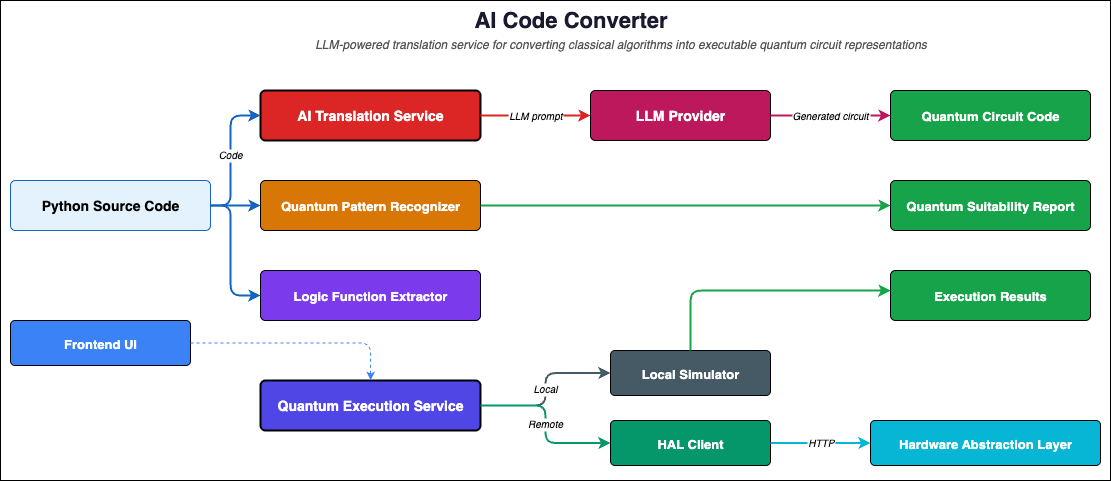
\includegraphics[width=0.85\textwidth]{ai-code-convertor.png}
\caption{AI Code Converter pipeline}
\label{fig:ai-code-converter}
\end{figure}

\subsection{Supported Transformations}
The converter targets well-established algorithm mappings: linear search to Grover's algorithm, hidden bitstring discovery to Bernstein--Vazirani, parity checking to Deutsch's algorithm, classical swap to quantum swap, state transfer to quantum teleportation, period finding to QFT-based routines, and factoring to Shor's algorithm. These were selected because the quantum counterparts are known, teachable, and suitable for controlled validation.

\subsection{AST Compatibility Scoring}
Before conversion, a Python AST analyser extracts structural patterns such as loops, conditionals, arithmetic operations, function calls, and bitwise operations. These features are matched against a pattern database to compute a compatibility score for each supported algorithm category. This module is independent of the language model, making it an interpretable filter before expensive or misleading conversion attempts.

\subsection{CodeT5 Conversion}
The conversion model is a fine-tuned CodeT5-base model trained on curated Python-to-Qiskit pairs. Input code is normalised and tokenised, and the model generates Qiskit circuits using beam-search decoding. Generated code is then validated syntactically and through Qiskit Aer simulation where applicable.

\subsection{Training Configuration}
The converter training process used supervised sequence-to-sequence fine-tuning on curated source-target pairs. Training included checkpoint monitoring, validation-loss tracking, and stopping decisions based on stable convergence. Tokenization strategy and output length constraints were selected to accommodate circuit-construction idioms common in Qiskit outputs.

Model quality was evaluated through multiple complementary metrics rather than exact match only. This is necessary because semantically equivalent circuit implementations can differ in register naming, gate order, decomposition style, and formatting.

\subsection{Conversion Safety and Reliability Controls}
Conversion requests include compatibility assessment before generation. Low-confidence or unsupported patterns are flagged to prevent misleading transformations. Generated outputs pass syntax checks and simulation-oriented sanity checks where applicable. This two-step guardrail (compatibility then generation validation) reduces the risk of invalid quantum code being forwarded to execution services.

\subsection{Human-in-the-Loop Use Pattern}
Although automated conversion is provided, the tool is intended for assisted development rather than unquestioned replacement of domain expertise. The report output is designed to support review by exposing compatibility, predicted algorithm family, and performance context. This allows users to accept, modify, or reject generated code responsibly.

\section{Decision Engine}
The Decision Engine is the routing intelligence of Nexar. It combines three decision sources: ML-based prediction, rule-based validation, and cost analysis.

\begin{figure}[H]
\centering
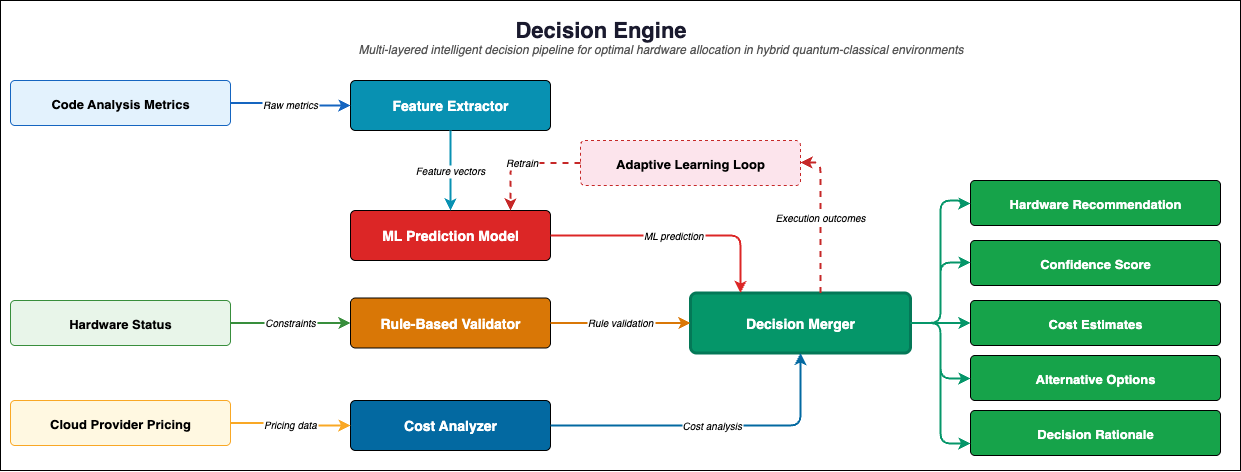
\includegraphics[width=0.85\textwidth]{decision-engine.png}
\caption{Decision Engine architecture}
\label{fig:decision-engine}
\end{figure}

\subsection{Feature Vector}
The Decision Engine consumes a 16-feature vector consisting of 10 raw analysis features and 6 derived physics-aware features. The derived features are shown in Table \ref{tab:derived-features}.

\begin{table}[H]
\centering
\caption{Derived physics-aware features}
\label{tab:derived-features}
\begin{tabular}{p{0.28\textwidth}p{0.32\textwidth}p{0.28\textwidth}}
\toprule
\textbf{Feature} & \textbf{Formula} & \textbf{Purpose} \\
\midrule
Circuit volume & Qubits $\times$ depth & Resource intensity \\
Noise sensitivity & Qubits $\times$ depth $\times$ CX ratio & Error accumulation \\
Quantum overhead ratio & Problem size / qubits & Encoding efficiency \\
NISQ viability score & Composite threshold penalty & Current-hardware feasibility \\
Gate density & Gate count / qubits & Operational complexity \\
Entanglement factor & CX ratio $\times$ entanglement score & Entanglement signal \\
\bottomrule
\end{tabular}
\end{table}

\subsection{Two-Stage Routing Pipeline}
The first stage is a deterministic rule engine. It can force classical execution, force quantum execution, reject an infeasible workload, or allow both options. Force rules handle unambiguous regimes such as workloads with no quantum structure, circuits exceeding provider qubit limits, and circuits beyond classical state-vector simulation feasibility. The second stage handles ambiguous \texttt{ALLOW\_BOTH} workloads through weighted voting:

\begin{equation}
S_{\text{quantum}} = 0.50P_{\text{ML}} + 0.35P_{\text{rules}} + 0.15P_{\text{cost}}
\end{equation}

The weighting gives the ML model the largest influence in ambiguous cases, preserves rule influence for physical constraints, and uses cost as a tie-breaker because cloud pricing changes over time.

\subsection{Rule System Design Principles}
The rule layer encodes physical necessity, safety constraints, and known infeasibility boundaries. Rules are designed to be interpretable and auditable. They explicitly prioritize hard feasibility over statistical preference. For example, oversized workloads beyond backend constraints are rejected regardless of ML probability. Conversely, workloads with no quantum structure are forced to classical execution.

Rule configuration is externalizable so that threshold tuning can occur without deep service rewrites. This supports future calibration as hardware characteristics evolve.

\subsection{ML Calibration and Confidence Use}
Confidence calibration is essential because routing decisions combine signals from heterogeneous sources. Uncalibrated probabilities can cause one component to dominate inappropriately. Platt-style calibration was used to improve confidence reliability for downstream weighted merging. The calibrated confidence is used as a decision support signal rather than sole authority.

\subsection{Cost-Aware Trade-Off Modeling}
The cost component is intentionally lower-weighted due to pricing volatility and differences in billing semantics across providers. Its role is to discourage economically poor quantum choices in ambiguous regimes without overriding hard feasibility constraints. This design prevents price snapshots from destabilizing the routing policy.

\subsection{Cost Model}
The quantum cost model follows IBM pay-as-you-go QPU-second pricing:

\begin{equation}
C_q = t_q \times r_{\text{QPU}}
\end{equation}

where $t_q$ is billable QPU reservation time and $r_{\text{QPU}}$ is USD 1.60 per QPU-second for the pricing epoch used in the study. The classical cost model estimates compute time, memory usage, and fixed submission overhead for AWS EC2-style execution:

\begin{equation}
C_c = t_c r_{\text{compute}} + M_{\text{GB}}t_c r_{\text{memory}} + C_{\text{overhead}}
\end{equation}

\subsection{Decision Explainability Output}
Each decision response includes not only the final route but also explanatory signals: component-level tendencies, confidence summary, and key feature cues. This output is intended to support educational and operational transparency. Explainability is especially important in edge cases where users expect quantum routing but receive classical recommendations due to depth or viability constraints.

\section{Hardware Abstraction Layer}
The Hardware Abstraction Layer provides a unified execution interface across quantum and classical compute providers.

\begin{figure}[H]
\centering
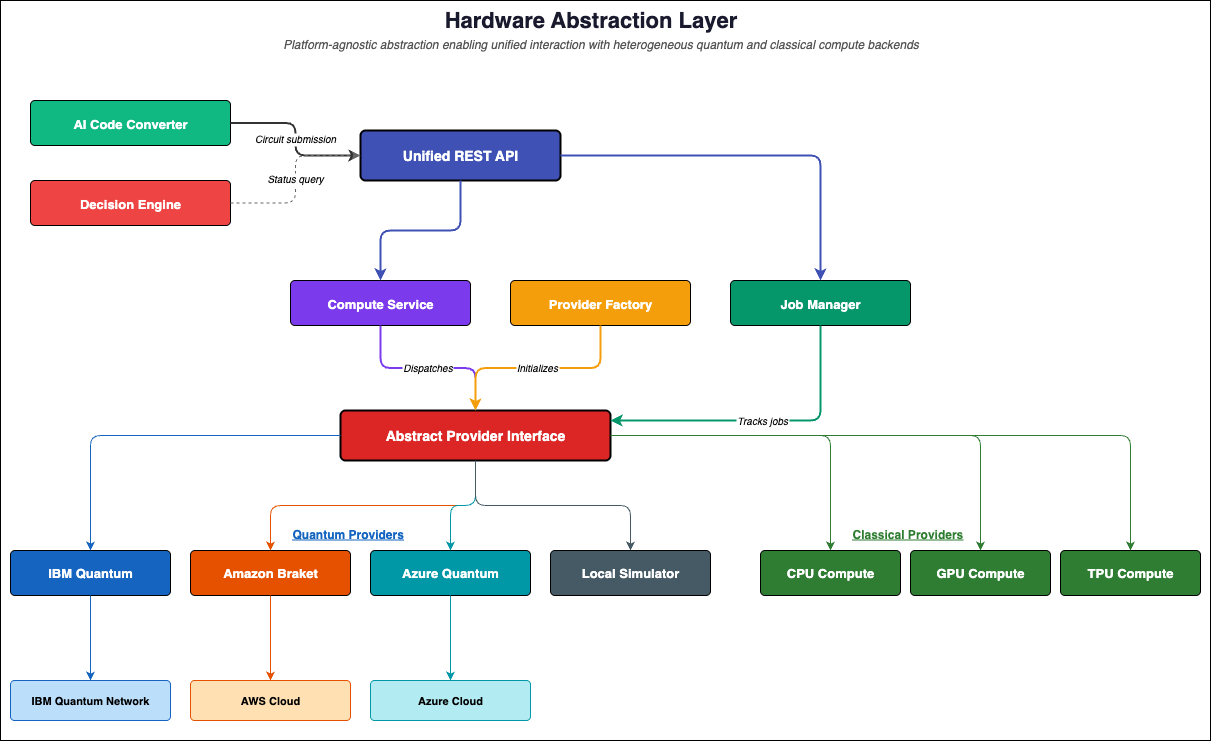
\includegraphics[width=0.85\textwidth]{hardware-abstraction.png}
\caption{Hardware Abstraction Layer architecture}
\label{fig:hardware-abstraction}
\end{figure}

\subsection{Provider Architecture}
The HAL uses a factory-based provider architecture with common abstract interfaces for all providers. \texttt{BaseProvider} defines common lifecycle methods such as device listing, job status, result retrieval, and batch execution. \texttt{QuantumProvider} extends this contract for circuit execution, while \texttt{ClassicalProvider} extends it for task execution. IBM Quantum is fully implemented, while AWS Quantum, Azure Quantum, and several classical providers are scaffolded behind the same interface.

\subsection{Job Lifecycle Management}
The HAL implements a job lifecycle covering pending, queued, scheduled, submitted, running, completed, failed, cancelled, and queued-unavailable states. Redis is used for persistent job state in production, with an in-memory fallback for development and CI environments. Google Cloud Pub/Sub publishes job updates for distributed notification.

\subsection{Sandboxed Python Execution}
The HAL includes a sandboxed Python execution endpoint for Qiskit circuits. It restricts built-ins, enforces an import allowlist, validates the presence of a \texttt{QuantumCircuit}, and applies timeout protection. Tests confirmed that attempts to access files or import modules such as \texttt{os}, \texttt{socket}, and \texttt{subprocess} are rejected.

\subsection{Provider Extensibility Strategy}
Providers are registered through a common contract and factory initialization. This allows incremental onboarding of new backends without changing gateway or decision code paths. The architecture is designed so that provider-specific complexity stays confined to provider modules, while the rest of the system remains backend-agnostic.

\subsection{Execution Observability}
Job status transitions are emitted as structured updates suitable for dashboards and asynchronous consumers. This observability layer supports tracing, user-facing status updates, and post-run analysis. Combined with request identifiers from the gateway, it enables end-to-end request lineage across services.

\section{Deployment Methodology}
All six services are containerised and deployed on Google Cloud Run. Docker images are stored in Artifact Registry, and Terraform manages Cloud Run services, IAM, Artifact Registry, and supporting resources. GitHub Actions automates build and deployment workflows. This architecture allows each service to scale independently and supports service-by-service release management.

\subsection{CI/CD Workflow Overview}
The CI/CD flow performs dependency installation, static checks, test execution, image build, artifact publishing, and deployment. Service-level pipelines allow independent release cadence. This is important because model-heavy services and frontend services have different deployment risks and rollback needs.

\subsection{Operational Monitoring Considerations}
Production operations require latency, error-rate, queue-depth, and provider-status visibility. The current system includes structured logs and service-level health endpoints. Future operational maturity should include centralized dashboards, SLO thresholds, and automated incident notification flows.

\section{Commercialisation Aspects}
Nexar has commercial potential as a routing and orchestration layer for organisations experimenting with quantum computing. Target users include research laboratories, universities, enterprise early adopters in finance and logistics, and quantum software vendors. Possible revenue models include a hosted SaaS routing layer, on-premises deployments for private workloads, usage-based API billing, and consulting for custom routing policies or provider integration.

\subsection{Target Audience Segments}
The first segment is academic and research institutions requiring affordable experimentation workflows without deep in-house quantum engineering capabilities. The second segment is enterprise innovation teams exploring selective quantum use cases in optimization, simulation, and cryptography-adjacent research. The third segment is platform vendors seeking pluggable routing intelligence to enhance existing compute orchestration offerings.

\subsection{Value Proposition}
Nexar provides value by reducing decision uncertainty and integration burden. Instead of requiring each team to build analysis and routing logic from scratch, Nexar offers reusable intelligence and execution abstraction. This lowers onboarding time, improves governance consistency, and reduces avoidable quantum spend from unsuitable routing.

\subsection{Business Models}
Potential commercialization models include:
\begin{enumerate}
\item Subscription SaaS model with tiered request quotas and advanced analytics features.
\item Enterprise deployment model with private network integration, custom policy controls, and support SLAs.
\item Usage-based API billing model for high-variability workloads.
\item Professional services model for provider integration, policy tuning, and regulated-environment deployment.
\end{enumerate}

\subsection{Market and Adoption Risks}
Key adoption risks include rapid provider API evolution, fluctuating pricing models, unclear near-term ROI expectations, and trust barriers in automated routing decisions. Mitigations include clear explainability outputs, extensible provider modules, and continuous calibration with empirical execution traces.

\subsection{Commercial Readiness Roadmap}
Commercial readiness requires hardening in four areas: multi-provider completion, security posture uplift, observability and SLA tooling, and contractual deployment support. A phased roadmap can start with academic/innovation pilot deployments and progress to enterprise integrations once backend diversity and operational reliability targets are met.

\section{Testing and Implementation}
Testing was performed at component and integrated levels. Component tests covered model evaluation, AST parsing, API schemas, conversion quality, sandbox restrictions, provider registration, Redis fallback, scheduling, and IBM Quantum job submission. Integrated evaluation used a 100-workload benchmark, pipeline latency measurement, cost comparison, and 27 real IBM Quantum hardware runs.

\subsection{Testing Strategy}
Testing follows a layered strategy:
\begin{enumerate}
\item Unit tests validate deterministic logic and parser behaviour.
\item Component tests validate service-level responses and model outputs.
\item Integration tests validate cross-service request flow through the gateway.
\item System tests validate end-to-end routing and execution outcomes.
\item Benchmark and hardware tests validate performance and practical viability.
\end{enumerate}

\subsection{Representative Unit and Component Tests}
Representative tests include AST branch counting validation, language classifier inference schema validation, converter syntax checks, rule-engine threshold behaviour tests, cost-model arithmetic checks, provider registration validation, and sandbox security rejection cases. These tests reduce regression risk when models or provider code paths evolve.

\subsection{Integration and End-to-End Validation}
End-to-end tests submit workload samples through gateway APIs and verify complete lifecycle behaviour: analysis response, routing decision, conversion where applicable, execution submission, status polling, and result retrieval. This validates not only individual services but also contract compatibility and orchestration reliability.

\subsection{Benchmark and Hardware Validation Protocol}
The benchmark protocol uses 100 workloads with mixed classical, hybrid, and quantum categories. Routing outcomes are compared against dual oracles, and additional diagnostics include weight sensitivity and latency profiles. Hardware validation uses IBM backend submissions to verify that recommended quantum paths are operationally executable.

\subsection{Quality Assurance Artifacts}
Quality assurance artefacts include evaluation tables, confusion matrices, calibration curves, routing summaries, timing tables, and hardware-result logs. These artefacts provide traceable evidence for each major claim in the results chapter.

\subsection{Implementation Milestones}
Implementation progressed in stages: architecture definition, component prototyping, model training and evaluation, service integration, benchmark evaluation, and hardware validation. This staged approach allowed risk containment and clearer attribution of issues to specific pipeline layers.

\chapter{RESULTS AND DISCUSSION}

\section{Code Analysis Engine Results}
The Code Analysis Engine achieved strong performance in language classification and practical performance in algorithm classification. The ensemble language classifier achieved 98.52\% accuracy on 1,080 held-out samples. Q\# reached perfect precision and recall, while Qiskit was the most difficult class due to its overlap with generic Python.

\begin{table}[H]
\centering
\caption{Code Analysis Engine language-classifier results}
\begin{tabular}{lr}
\toprule
\textbf{Metric} & \textbf{Value} \\
\midrule
Accuracy & 98.52\% \\
Macro precision & 98.59\% \\
Macro recall & 98.66\% \\
Macro F1 & 98.62\% \\
Weighted F1 & 98.52\% \\
\bottomrule
\end{tabular}
\end{table}

The single-algorithm classifier achieved 86.39\% accuracy over 8,800 samples across ten algorithm classes. QAOA, QPE, Shor, Simon, and VQE were classified perfectly or near-perfectly because their circuit patterns are distinctive. Grover, Deutsch--Jozsa, Bernstein--Vazirani, and QFT showed more confusion because they share oracle-style or transform-style structures. The experimental multi-label classifier reached F1-micro of 0.3976, exposing the need for larger balanced multi-algorithm datasets.

\subsection{Interpretation of CAE Results}
The language-classification result indicates that framework detection is production-usable in this context. Error concentration in Qiskit versus generic Python classes is expected because framework code remains syntactically valid Python. The algorithm-classification result is sufficient for routing support but not yet robust enough for fully autonomous algorithm governance without confidence thresholds.

\subsection{Observed Error Modes}
Common CAE error modes include ambiguous oracle-style circuits and short snippets lacking clear structural signatures. In these cases, deterministic pattern checks reduce but do not eliminate ambiguity. These observations support investment in richer semantic representations and larger real-world datasets.

\section{AI Code Converter Results}
The AI Code Converter was evaluated on 300 held-out samples across the supported transformation families. Exact match was low because multiple Qiskit implementations can be functionally equivalent without matching character-for-character. Syntactic validity and algorithm-family correctness are more meaningful for code generation.

\begin{table}[H]
\centering
\caption{AI Code Converter evaluation results}
\begin{tabular}{lr}
\toprule
\textbf{Metric} & \textbf{Value} \\
\midrule
Valid Qiskit circuit rate & 98.7\% \\
Correct algorithm type & 77.7\% \\
BLEU score & 28.36 \\
Exact match & 19.7\% \\
Token precision, secondary run & 95.88\% \\
Token F1, secondary run & 68.85\% \\
\bottomrule
\end{tabular}
\end{table}

Generated circuits for all supported categories were executed on Qiskit Aer under ideal and noise-model conditions. Grover circuits showed the expected target-state amplification, Bernstein--Vazirani circuits recovered hidden bitstrings in one query, Deutsch circuits identified parity, QFT circuits produced expected Fourier-domain outputs, and small Shor circuits produced period-finding measurements consistent with expected factors.

\subsection{Interpretation of Conversion Metrics}
The high valid-circuit rate confirms that the model learns Qiskit syntax reliably. Lower exact-match values reflect representational diversity rather than wholesale conversion failure. Algorithm-type correctness and simulation behaviour provide stronger evidence of practical conversion utility than token identity metrics alone.

\subsection{Failure Cases and Practical Safeguards}
Failure cases generally involve unsupported patterns, atypical code organization, or transformations requiring richer semantic context than current prompts capture. The compatibility scoring gate and post-generation validation act as safeguards that prevent most low-quality conversions from reaching execution services.

\section{Decision Engine Results}
The Decision Engine's calibrated Random Forest achieved 97.72\% accuracy on an 876-sample synthetic held-out split, with XGBoost and Gradient Boosting achieving 98.40\% and 98.29\% respectively. The production model selection favoured calibration and interpretability rather than only raw accuracy.

\begin{table}[H]
\centering
\caption{Decision Engine ML model performance on held-out synthetic data}
\begin{tabular}{lrrrr}
\toprule
\textbf{Model} & \textbf{Accuracy} & \textbf{Macro F1} & \textbf{ROC-AUC} & \textbf{Brier} \\
\midrule
Random Forest & 0.9772 & 0.9772 & 0.9987 & 0.0156 \\
XGBoost & 0.9840 & 0.9840 & 0.9986 & 0.0136 \\
Gradient Boosting & 0.9829 & 0.9829 & 0.9977 & 0.0129 \\
\bottomrule
\end{tabular}
\end{table}

The more important integrated evaluation uses 100 real benchmark workloads and two oracles. Oracle A labels workloads by theoretical algorithmic advantage. Oracle B labels workloads by hardware viability under present NISQ constraints. Because the benchmark is class-imbalanced, F1(Q) and Cohen's kappa are more informative than accuracy.

\begin{table}[H]
\centering
\caption{Routing accuracy against dual-oracle benchmark}
\begin{tabular}{lrrrr}
\toprule
\textbf{Oracle} & \textbf{Accuracy} & \textbf{Precision(Q)} & \textbf{Recall(Q)} & \textbf{F1(Q)} \\
\midrule
Oracle A: Algorithmic advantage & 0.810 & 0.381 & 0.571 & 0.457 \\
Oracle B: Hardware viability & 0.860 & 0.333 & 1.000 & 0.500 \\
\bottomrule
\end{tabular}
\end{table}

The results show that Nexar is conservative in the expected direction. It avoids routing many small or deep circuits to quantum hardware because present-day hardware noise and cost make classical execution more practical. Under Oracle B, Nexar recovers every true Quantum workload, achieving perfect Quantum-class recall, though precision remains limited because some quantum recommendations are false positives under the strict hardware-viability oracle.

\subsection{Synthetic-to-Real Gap Analysis}
The contrast between high synthetic held-out accuracy and lower real benchmark separability is a central finding. It highlights the limits of synthetic training distributions for practical routing. The two-stage architecture partly compensates for this gap by embedding hard feasibility constraints independent of learned representations.

\subsection{Ablation and Stability Insights}
Weight sensitivity and component ablation analyses show that deterministic constraints dominate in physically unambiguous regions, while ML influence matters most in ambiguous regimes. Cost acts as a moderating factor. This behaviour is consistent with the design intent of the weighted architecture.

\section{Weight Sensitivity}
Weight sensitivity analysis showed that the baseline 50/35/15 weighting is stable across reasonable alternatives. ML-heavy, rule-heavy, and cost-sensitive configurations produced identical routing counts for the 100-workload benchmark. Only adversarial equal weighting with cost as the largest component caused substantial routing changes.

\begin{table}[H]
\centering
\caption{Weight sensitivity summary}
\begin{tabular}{lrrr}
\toprule
\textbf{Weights (ML/Rules/Cost)} & \textbf{Quantum} & \textbf{Classical} & \textbf{Changed vs. baseline} \\
\midrule
50/35/15 & 20 & 80 & -- \\
70/20/10 & 20 & 80 & 0 \\
30/55/15 & 20 & 80 & 0 \\
40/30/30 & 20 & 80 & 0 \\
100/0/0 & 18 & 82 & 2 \\
33/33/34 & 46 & 54 & 26 \\
\bottomrule
\end{tabular}
\end{table}

\section{Cost Analysis Results}
The cost analysis confirms that present-day quantum execution is not economically preferable for small workloads. Classical execution is approximately USD 0.001 for representative workloads, while quantum-routed workloads range from USD 0.375 to USD 1.578 under the IBM QPU-second pricing model used in the study.

\begin{table}[H]
\centering
\caption{Representative cost comparison}
\begin{tabular}{lrrr}
\toprule
\textbf{Workload} & \textbf{Qubits} & \textbf{Target} & \textbf{Estimated cost (USD)} \\
\midrule
FFT signal processing & 0 & Classical & 0.001 \\
Sorting suite & 0 & Classical & 0.001 \\
QAOA graph partition & 20 & Quantum & 0.439 \\
QAOA MaxCut & 50 & Quantum & 0.917 \\
Iron-sulfur VQE & 60 & Quantum & 1.421 \\
120-qubit VQE & 120 & Quantum & 1.578 \\
\bottomrule
\end{tabular}
\end{table}

The decisive crossover is not a smooth cost equality point, but a physical feasibility boundary. Full state-vector simulation requires $2^n$ complex amplitudes. At 50 qubits this approaches 16 PB of memory, and at 60 qubits it approaches 16 EB. Beyond this range, exact classical simulation of high-entanglement circuits becomes infeasible regardless of nominal cloud pricing.

\subsection{Economic Interpretation}
Current economics indicate that quantum execution should be used selectively in the NISQ era. For small and medium workloads, classical paths remain strongly preferable unless specialized quantum objectives justify additional cost. Cost-aware routing is therefore not optional; it is a practical requirement to prevent unsustainable execution policy.

\begin{figure}[H]
\centering
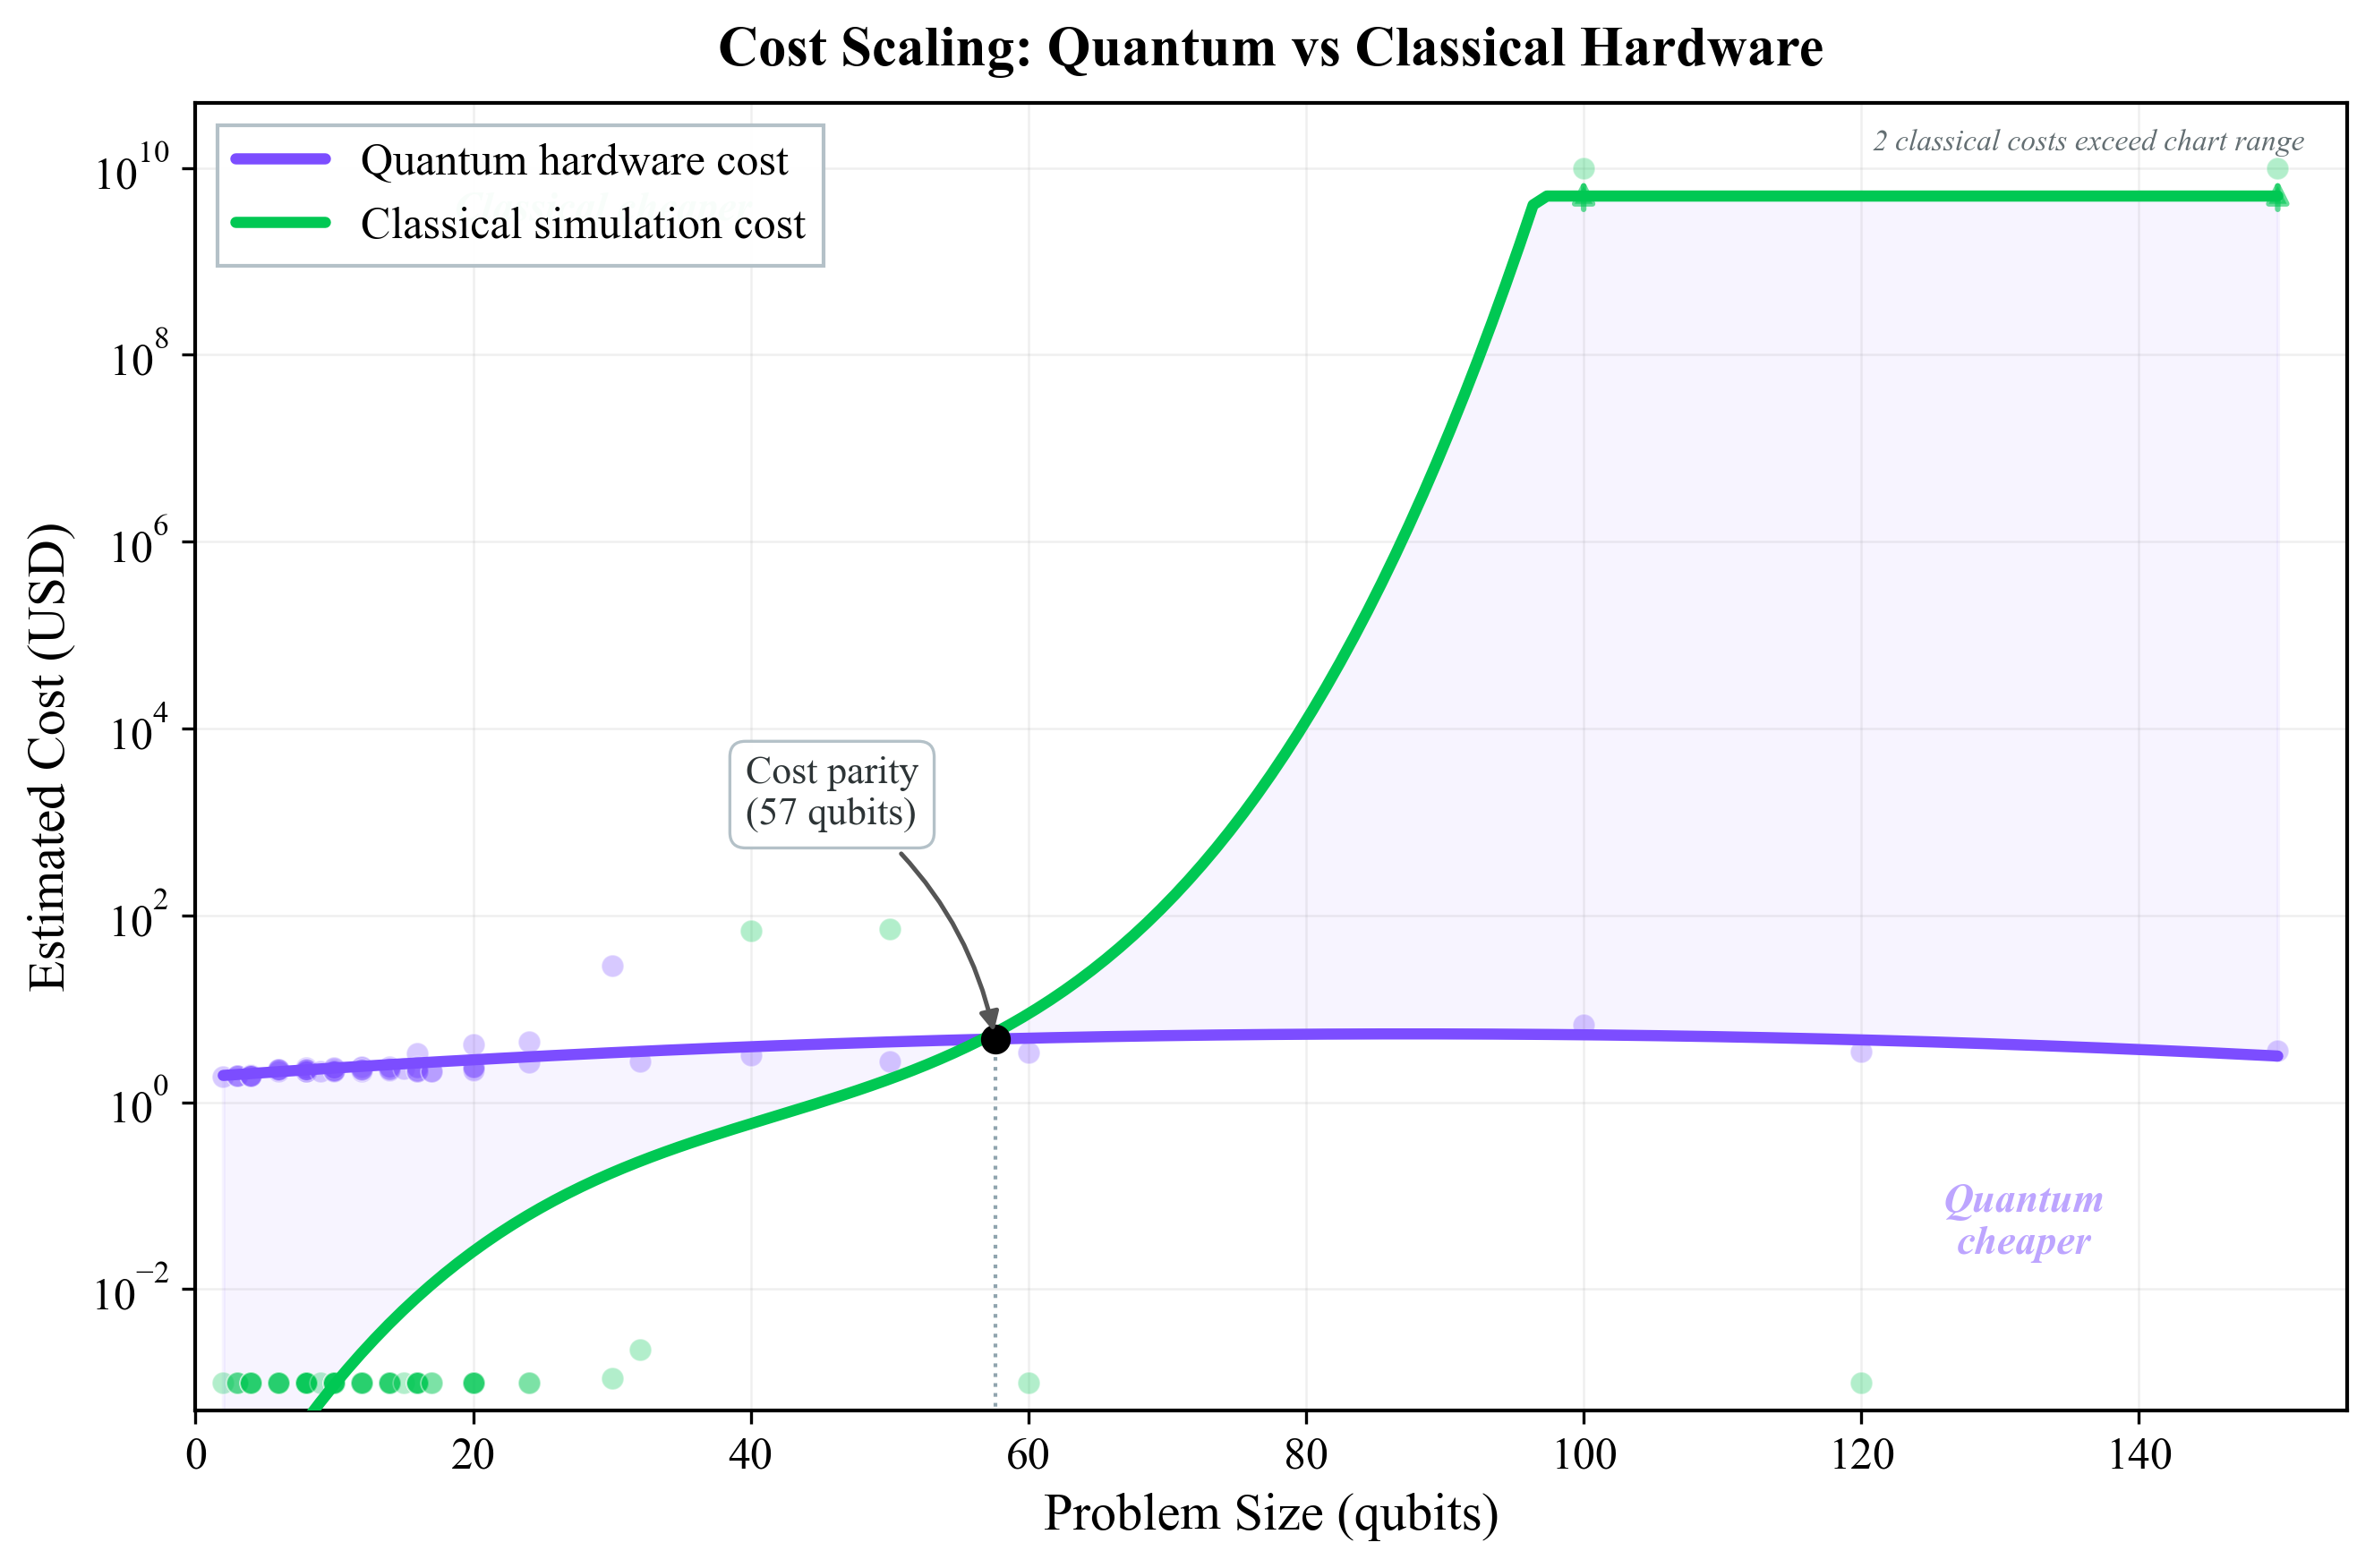
\includegraphics[width=0.85\textwidth]{cost-scaling.png}
\caption{Quantum and classical cost-scaling crossover}
\label{fig:cost-scaling}
\end{figure}

\section{Pipeline Performance}
Warm pipeline latency averaged approximately 1.5 seconds end-to-end. Quantum workloads required longer analysis time because the Code Analysis Engine performs additional circuit parsing and quantum metric extraction. Decision latency remained below 15 ms, showing that routing itself is not the system bottleneck.

\begin{table}[H]
\centering
\caption{Pipeline timing metrics}
\begin{tabular}{lrr}
\toprule
\textbf{Metric} & \textbf{Classical path} & \textbf{Quantum path} \\
\midrule
Average analysis time & 731 ms & 1,355 ms \\
Average decision time & 12 ms & 10 ms \\
Average total pipeline time & 1,222 ms & 1,770 ms \\
Language detection confidence & 0.942 & 0.966 \\
\bottomrule
\end{tabular}
\end{table}

\section{Hardware Abstraction Layer Results}
The HAL successfully registered 10 provider interfaces and returned device listings through a unified API. IBM Quantum integration was validated through simulator and real-device execution. A Bell-state circuit submitted to the IBM Aer simulator completed in approximately 3 seconds and returned the expected balanced counts for \texttt{00} and \texttt{11}. Real IBM backend submission was also validated, though queue duration varied by backend availability.

Calibration extraction returned metrics such as median two-qubit gate error, single-qubit gate error, readout error, T1, T2, and gate time. Calibration caching reduces repeated device-listing overhead from potentially tens of seconds to less than 500 ms for repeated requests.

Batch execution improved submission overhead. Five circuits submitted sequentially required approximately 2.5 seconds and five job IDs, while a single batched submission required approximately 0.7 seconds and one composite job ID, a 3.6x reduction in submission overhead.

\subsection{Operational Interpretation}
HAL results demonstrate that abstraction overhead can remain manageable while preserving extensibility. The batch-path gains show clear operational value for repeated circuit submissions. Device metadata exposure and status lifecycle management improve operability for both users and system maintainers.

\section{Real Hardware Validation}
The project validated 27 circuits on IBM hardware through the HAL. The results support the router's NISQ-aware behaviour. Shallow circuits such as Deutsch--Jozsa, Bernstein--Vazirani, and small QPE produced high-fidelity outputs. Deeper circuits, even with few qubits, degraded strongly. Large circuits such as 50-qubit QAOA, 60-qubit iron-sulfur VQE, and 120-qubit VQE were successfully dispatched, but produced noise-dominated outputs, which is expected without error mitigation or fault-tolerant hardware.

\begin{table}[H]
\centering
\caption{Selected real-hardware validation results}
\begin{tabular}{lrrrl}
\toprule
\textbf{Circuit} & \textbf{Qubits} & \textbf{Depth} & \textbf{Top outcome \%} & \textbf{Nexar route} \\
\midrule
Deutsch--Jozsa constant & 2 & 3 & 99.9 & Classical \\
Bernstein--Vazirani & 4 & 9 & 96.3 & Classical \\
QPE T gate & 4 & 80 & 82.3 & Classical \\
Grover search & 4 & 241 & 33.5 & Classical \\
QAOA graph partition & 20 & 398 & 0.1 & Quantum \\
ZNE benchmark & 24 & 1 & 68.5 & Quantum \\
QAOA MaxCut & 50 & 580 & 0.1 & Quantum \\
Iron-sulfur VQE & 60 & 242 & 0.1 & Quantum \\
120-qubit VQE & 120 & 482 & 0.1 & Quantum \\
\bottomrule
\end{tabular}
\end{table}

The main hardware finding is that post-transpile depth predicts fidelity more reliably than qubit count alone. Circuits below approximately depth 80 produced strong results, while circuits above roughly depth 130 tended toward the noise floor. This supports the Decision Engine's use of NISQ viability and circuit-depth thresholds.

\subsection{Practical Implications for Routing Policy}
Hardware validation confirms that a naive ``qubit count only'' policy is insufficient. Routing policies must account for transpiled depth and noise context to avoid overconfident quantum recommendations. This supports future work on integrating richer backend calibration signals directly into decision-time viability scoring.

\section{Research Findings}
The first finding is that integrated routing is necessary. Code analysis, conversion, routing, and execution each solve part of the problem, but the user value appears when all four are connected into one workflow.

The second finding is that language detection is mature enough for practical use in this domain. The Code Analysis Engine's 98.52\% accuracy makes it reliable as the first stage of the pipeline.

The third finding is that algorithm classification and code conversion are feasible but dataset-limited. Single-algorithm recognition achieved useful accuracy, while multi-label recognition and broader conversion need larger, more diverse real-world code corpora.

The fourth finding is that rule-based physics constraints remain essential. Synthetic ML performance is high, but real benchmark performance drops, so deterministic constraints are needed to keep routing safe and explainable.

The fifth finding is that cost currently favours classical execution for small and medium workloads. Quantum execution becomes necessary mainly when classical simulation becomes physically infeasible or when a workload falls into a practical NISQ advantage regime.

The sixth finding is that provider abstraction is necessary for maintainability. The HAL allows routing and analysis components to remain independent of provider-specific SDKs, enabling future expansion to AWS Braket and Azure Quantum.

\section{Discussion by Research Objectives}
\subsection{Objective 1: Multi-Language Code Analysis}
The project achieved objective one with high language-classification performance and operationally useful algorithm/complexity extraction. Remaining work concerns multi-label robustness and complete canonical IR adoption.

\subsection{Objective 2: Automated Code Conversion}
Objective two was achieved within scoped algorithm families. The converter is practically useful in assisted workflows but should not yet be treated as universal conversion automation.

\subsection{Objective 3: Decision Intelligence}
Objective three was achieved through the two-stage decision architecture and dual-oracle evaluation. The route-selection logic is transparent and conservative, matching NISQ operational realities.

\subsection{Objective 4: Provider-Agnostic Execution}
Objective four was achieved architecturally and partially empirically. IBM execution is validated in depth; AWS and Azure provider paths require completion for full empirical parity.

\subsection{Objective 5: Integrated Platform}
Objective five was achieved through microservice orchestration with deployable infrastructure and documented service contracts. The platform demonstrates coherent end-to-end flow from code submission to result delivery.

\subsection{Objective 6: Empirical Evaluation}
Objective six was achieved through held-out model evaluations, benchmark routing analysis, latency profiling, cost studies, and real-hardware runs. Statistical breadth can be increased in future work through expanded workload sets and repeated longitudinal evaluations.

\section{Summary of Each Student's Contribution}
\begin{longtable}{p{0.22\textwidth}p{0.68\textwidth}}
\caption{Summary of student contributions} \\
\toprule
\textbf{Student} & \textbf{Contribution} \\
\midrule
Jayasinghe Y L (IT22103840) & Designed and implemented the Code Analysis Engine, including multi-language detection, classical AST complexity analysis, quantum metric extraction, algorithm classification, Canonical IR exploration, FastAPI integration, and frontend analysis visualisation. \\
\addlinespace
Hettiarachchi S R (IT22128386) & Designed and implemented the AI Code Converter, including AST compatibility scoring, CodeT5-based Python-to-Qiskit generation, performance prediction with Qiskit Aer, REST API integration, and validation across supported algorithm mappings. \\
\addlinespace
Prasad H G A T (IT22056870) & Designed and implemented the Decision Engine, including feature engineering, calibrated ML routing model, physics-aware rule system, cost analyser, weighted merger, benchmark evaluation, sensitivity analysis, and routing audit outputs. \\
\addlinespace
Siriwardhana A H L T S (IT22094568) & Designed and implemented the Hardware Abstraction Layer, including provider abstraction, IBM Quantum integration, job lifecycle management, Redis persistence, Pub/Sub messaging, sandboxed Qiskit execution, calibration extraction, and provider extensibility scaffolding. \\
\bottomrule
\end{longtable}

\section{Limitations}
Several limitations remain. The Decision Engine ML model shows a synthetic-to-real gap, meaning future training should use execution traces from production hardware. The AI Code Converter supports a focused set of algorithms rather than general-purpose conversion. The Code Analysis Engine's multi-label classifier is not yet production-ready because current datasets are too small and imbalanced. Real-hardware validation was performed on IBM hardware only, while AWS Braket and Azure Quantum remain architectural scaffolds. Provider pricing is static for the evaluation period and should be replaced by live pricing integration. Finally, NISQ hardware noise limits the fidelity of deep circuits, so future routing should incorporate error mitigation and fault-tolerant hardware assumptions as the ecosystem matures.

\section{Threats to Validity}
\subsection{Internal Validity}
Internal validity risks include dataset curation bias, synthetic-sample distribution effects, and implicit assumptions in rule thresholds. Mitigation included held-out testing, ablation studies, and explicit threshold documentation.

\subsection{External Validity}
External validity is limited by provider coverage and benchmark size. Although workload diversity is broad, conclusions may shift under different workload distributions, provider pricing epochs, or hardware generations.

\subsection{Construct Validity}
Construct validity depends on chosen quality metrics. Exact match is weak for code conversion compared with functional equivalence. Accuracy alone is weak for imbalanced routing classes; therefore F1(Q), kappa, and hardware observations are emphasized.

\subsection{Conclusion Validity}
Conclusion validity risks include small positive-class counts in some benchmark slices. Weight sensitivity and cross-component consistency reduce overinterpretation risk, but larger repeated studies are still required for stronger statistical confidence.

\chapter{CONCLUSION AND RECOMMENDATIONS}

\section{Conclusion}
This dissertation presented Nexar, an intelligent quantum-classical workload routing platform that integrates source-code analysis, classical-to-quantum conversion, decision intelligence, and provider-agnostic execution. The project demonstrates that practical hybrid orchestration can be built as a modular microservice system: the Code Analysis Engine identifies language, algorithm, and complexity; the AI Code Converter translates supported classical algorithms into Qiskit; the Decision Engine selects an execution target through ML, rules, and cost analysis; and the Hardware Abstraction Layer executes workloads through a unified provider interface.

The evaluation results show that Nexar meets the main objectives of the research. The Code Analysis Engine achieved 98.52\% language-classification accuracy and 86.39\% single-algorithm classification accuracy. The AI Code Converter generated syntactically valid Qiskit code for 98.7\% of held-out samples. The Decision Engine achieved 0.810--0.860 accuracy against two routing oracles, with perfect Quantum-class recall under the hardware-viability oracle. The HAL validated IBM Quantum execution, provider discovery, sandboxing, calibration extraction, job lifecycle management, and batch optimisation.

The broader conclusion is that quantum-classical routing should not be treated as a single ML classification problem. Current quantum hardware is constrained by cost, noise, depth, qubit availability, and simulator feasibility. Nexar's two-stage architecture reflects this reality: deterministic rules handle physical constraints, while ML and cost analysis contribute in ambiguous regimes. This architecture is practical for the NISQ era and extensible for future quantum hardware.

\section{Recommendations and Future Work}
Future work should prioritise retraining the Decision Engine on empirical execution traces from IBM hardware and, later, from AWS Braket and Azure Quantum. This will reduce the synthetic-to-real performance gap and support better calibration of routing confidence.

The AI Code Converter should be expanded beyond the current algorithm set to include variational quantum algorithms, quantum machine learning, and quantum chemistry workflows. Future evaluation should include output-distribution equivalence checks using fidelity or total variation distance rather than relying mainly on syntactic validity and token-overlap metrics.

The Code Analysis Engine should complete the Canonical IR implementation so that quantum metric extraction preserves qubit connectivity, control flow, and execution context more accurately than flat gate lists. Larger benchmark datasets are also required for reliable multi-label algorithm classification.

The Hardware Abstraction Layer should complete AWS Braket and Azure Quantum integrations, add production-grade hardware-isolated sandboxing, and move calibration caching to shared Redis storage for horizontally scaled deployments.

At platform level, Nexar should evolve toward multi-objective routing over cost, execution time, expected fidelity, carbon footprint, and user preference. As quantum hardware matures, the routing logic should also distinguish NISQ-era heuristics from fault-tolerant quantum computing assumptions.

\chapter{PROJECT EXECUTION AND GOVERNANCE}

\section{Project Planning and Work Breakdown}
The project followed a staged work breakdown structure spanning requirement analysis, architecture design, component implementation, model training, integration, and evaluation. Each stage produced concrete artefacts and review checkpoints. This structure reduced integration risk by aligning deliverables with service boundaries.

\section{Risk Management}
\subsection{Technical Risks}
Key technical risks included model underperformance, provider API instability, execution failures on cloud backends, and integration schema drift. Mitigations included fallback rules, schema validation, provider abstraction layers, and staged integration tests.

\subsection{Operational Risks}
Operational risks included deployment misconfiguration, secret management errors, and limited runtime observability. Mitigations included environment contracts, infrastructure-as-code practices, and health-check endpoints.

\subsection{Research Risks}
Research risks included overfitting to synthetic datasets and over-claiming practical quantum benefit. Mitigations included dual-oracle framing, hardware validation, explicit limitation reporting, and conservative interpretation of conversion metrics.

\section{Ethical, Security, and Social Considerations}
Automated routing systems can influence compute cost and trust decisions for users lacking deep domain expertise. Ethical practice therefore requires transparent explanations, conservative defaults, and explicit uncertainty communication. Security controls are required for code submission endpoints, especially where dynamic execution is involved. Socially, lowering quantum adoption barriers can broaden participation in advanced computing research and education.

\section{Maintainability and Future Team Handover}
Maintainability was supported through modular service boundaries, explicit contracts, and appendices documenting endpoint references and operational assumptions. Future handover should include model retraining procedures, provider onboarding checklists, and baseline benchmark rerun scripts to preserve continuity as team membership changes.

\chapter*{REFERENCES}
\addcontentsline{toc}{chapter}{References}
\begin{enumerate}
\item J. Preskill, ``Quantum computing in the NISQ era and beyond,'' \textit{Quantum}, vol. 2, p. 79, 2018.
\item P. W. Shor, ``Polynomial-time algorithms for prime factorization and discrete logarithms on a quantum computer,'' \textit{SIAM Journal on Computing}, vol. 26, no. 5, pp. 1484--1509, 1997.
\item L. K. Grover, ``A fast quantum mechanical algorithm for database search,'' in \textit{Proceedings of the 28th ACM Symposium on Theory of Computing}, 1996, pp. 212--219.
\item F. Arute et al., ``Quantum supremacy using a programmable superconducting processor,'' \textit{Nature}, vol. 574, pp. 505--510, 2019.
\item E. Farhi, J. Goldstone, and S. Gutmann, ``A quantum approximate optimization algorithm,'' arXiv:1411.4028, 2014.
\item A. Kandala et al., ``Hardware-efficient variational quantum eigensolver for small molecules and quantum magnets,'' \textit{Nature}, vol. 549, pp. 242--246, 2017.
\item IBM Quantum, ``Qiskit Runtime,'' 2023. [Online]. Available: \url{https://quantum.ibm.com/}
\item Amazon Web Services, ``Amazon Braket,'' 2023. [Online]. Available: \url{https://aws.amazon.com/braket/}
\item Microsoft, ``Azure Quantum,'' 2023. [Online]. Available: \url{https://azure.microsoft.com/en-us/products/quantum}
\item B. Weder, J. Barzen, F. Leymann, and M. Salm, ``Automated quantum hardware selection for quantum workflows,'' \textit{Electronics}, vol. 10, no. 8, p. 984, 2021.
\item A. JavadiAbhari et al., ``ScaffCC: Scalable compilation and analysis of quantum programs,'' \textit{Parallel Computing}, vol. 45, pp. 2--17, 2015.
\item Z. Feng et al., ``CodeBERT: A pre-trained model for programming and natural languages,'' in \textit{Findings of EMNLP}, 2020, pp. 1536--1547.
\item Y. Wang et al., ``CodeT5: Identifier-aware unified pre-trained encoder-decoder models for code understanding and generation,'' arXiv:2109.00859, 2021.
\item L. Breiman, ``Random forests,'' \textit{Machine Learning}, vol. 45, no. 1, pp. 5--32, 2001.
\item T. Chen and C. Guestrin, ``XGBoost: A scalable tree boosting system,'' in \textit{Proceedings of KDD}, 2016, pp. 785--794.
\item J. H. Friedman, ``Greedy function approximation: A gradient boosting machine,'' \textit{Annals of Statistics}, vol. 29, no. 5, pp. 1189--1232, 2001.
\item F. Pedregosa et al., ``Scikit-learn: Machine learning in Python,'' \textit{Journal of Machine Learning Research}, vol. 12, pp. 2825--2830, 2011.
\item FastAPI, ``FastAPI Documentation,'' 2023. [Online]. Available: \url{https://fastapi.tiangolo.com/}
\item Redis Ltd., ``Redis Documentation,'' 2023. [Online]. Available: \url{https://redis.io/docs/}
\item Google Cloud, ``Cloud Run Documentation,'' 2023. [Online]. Available: \url{https://cloud.google.com/run/docs}
\item Google Cloud, ``Cloud Pub/Sub Documentation,'' 2023. [Online]. Available: \url{https://cloud.google.com/pubsub/docs}
\item IBM Quantum, ``IBM Quantum pricing,'' 2024. [Online]. Available: \url{https://www.ibm.com/quantum/pricing}
\item Amazon Web Services, ``Amazon EC2 On-Demand Pricing,'' 2024. [Online]. Available: \url{https://aws.amazon.com/ec2/pricing/on-demand/}
\item K. Temme, S. Bravyi, and J. M. Gambetta, ``Error mitigation for short-depth quantum circuits,'' \textit{Physical Review Letters}, vol. 119, no. 18, p. 180509, 2017.
\end{enumerate}

\appendix
\chapter{Benchmark Workload Summary}
The integrated benchmark contains 100 workloads across classical, hybrid, and quantum categories. Classical workloads include sorting, dynamic programming, scientific computing, cryptography, machine learning, and graph problems. Hybrid workloads include VQE, QAOA, QSVM, QNN, transfer learning, and error-mitigation examples. Quantum workloads include Deutsch--Jozsa, Bernstein--Vazirani, Simon, QFT, QPE, Grover search, Shor factoring, QAOA, molecular simulation, and large VQE cases up to 120 qubits.

\section{Benchmark Category Detail}
\small
\begin{longtable}{p{0.26\textwidth}p{0.20\textwidth}p{0.44\textwidth}}
\toprule
\textbf{Category} & \textbf{Workload Count} & \textbf{Representative Workloads} \\
\midrule
Classical analytics & 12 & Sorting suites, matrix operations, dynamic programming benchmarks \\
Classical scientific & 10 & CFD-inspired loops, molecular dynamics kernels, numerical solvers \\
Classical ML & 10 & k-means, gradient boosting, classification pipelines, feature transforms \\
Hybrid variational & 12 & VQE chemistry variants, QAOA graph problems \\
Hybrid ML/mitigation & 11 & QSVM kernels, QNN circuits, transfer-learning style workloads, ZNE cases \\
Quantum foundational & 15 & Deutsch--Jozsa, Bernstein--Vazirani, Simon, QFT, QPE \\
Quantum search/factorization & 15 & Grover variants, Shor benchmarks \\
Quantum large-scale & 15 & 20q--120q circuits including QAOA and VQE families \\
\bottomrule
\end{longtable}
\normalsize

\section{Workload Metadata Fields}
For each workload, the benchmark records source type, detected language/framework, problem type, qubit requirement estimate, depth estimate, gate counts, runtime observations, routed target, confidence, and outcome metadata where execution occurred. This metadata supports both model diagnostics and auditability.

\chapter{Representative API Endpoints}
\begin{longtable}{>{\raggedright\arraybackslash}p{0.48\textwidth}>{\raggedright\arraybackslash}p{0.12\textwidth}>{\raggedright\arraybackslash}p{0.30\textwidth}}
\toprule
\textbf{Endpoint} & \textbf{Method} & \textbf{Purpose} \\
\midrule
\path|/api/v1/analysis/analyze| & POST & Analyse submitted source code \\
\path|/api/v1/decision/predict| & POST & Produce routing recommendation \\
\path|/api/v1/converter/translate| & POST & Convert supported Python code to Qiskit \\
\path|/api/v1/hardware/devices| & GET & List available execution devices \\
\path|/api/quantum/{provider}/execute| & POST & Submit quantum circuit job \\
\path|/api/quantum/jobs/{provider}/{id}| & GET & Retrieve quantum job status \\
\path|/api/quantum/jobs/{provider}/{id}/result| & GET & Retrieve quantum job result \\
\path|/api/classical/{provider}/execute| & POST & Submit classical execution task \\
\bottomrule
\end{longtable}

\chapter{Detailed Test Matrix}
\section{Unit and Component Test Cases}
\small
\begin{longtable}{p{0.14\textwidth}p{0.26\textwidth}p{0.20\textwidth}p{0.28\textwidth}}
\toprule
\textbf{Test ID} & \textbf{Target Component} & \textbf{Type} & \textbf{Expected Outcome} \\
\midrule
UT-CAE-01 & Language classifier input schema & Unit & Reject malformed payload with explicit validation error \\
UT-CAE-02 & AST branch counter & Unit & Deterministic cyclomatic count for known code sample \\
UT-CAE-03 & Quantum gate detector & Unit & Correctly detect gates in framework-specific snippet \\
UT-CAE-04 & Algorithm tier fallback & Component & Tier fallback occurs when confidence threshold unmet \\
UT-CONV-01 & Compatibility scorer & Unit & Unsupported pattern yields low compatibility score \\
UT-CONV-02 & Code generation syntax check & Component & Generated output parses as valid Python/Qiskit code \\
UT-CONV-03 & Conversion endpoint schema & Component & Valid request returns structured conversion response \\
UT-DEC-01 & Rule force classical & Unit & Non-quantum workload always forced classical \\
UT-DEC-02 & Rule reject oversized & Unit & Oversized qubit workload rejected deterministically \\
UT-DEC-03 & Weighted merge arithmetic & Unit & Composite score calculation matches formula \\
UT-DEC-04 & Cost-only tie-break behaviour & Component & Cost signal changes ambiguous decision as configured \\
UT-HAL-01 & Provider registry & Unit & Registered providers discoverable via API \\
UT-HAL-02 & Job state transition & Component & Valid transitions follow lifecycle contract \\
UT-HAL-03 & Queue unavailable flow & Component & Job moves to queued-unavailable then promoted on availability \\
UT-HAL-04 & Sandbox import block & Unit & Restricted modules rejected by sandbox policy \\
UT-HAL-05 & Sandbox timeout & Unit & Infinite loop interrupted at configured timeout \\
IT-001 & Gateway to CAE & Integration & Analysis payload returned with expected schema \\
IT-002 & Gateway to decision & Integration & Decision response includes route and confidence \\
IT-003 & Decision to converter gating & Integration & Conversion called only for supported route/path \\
IT-004 & Decision to HAL dispatch & Integration & Execution request accepted by selected provider path \\
IT-005 & Status polling loop & Integration & Status transitions visible through gateway path \\
IT-006 & Result retrieval chain & Integration & Final result retrievable and traceable by ID \\
E2E-001 & Classical workload full flow & End-to-end & Code analyzed, routed classical, executed, result returned \\
E2E-002 & Quantum workload full flow & End-to-end & Code analyzed, routed quantum, dispatched, result returned \\
E2E-003 & Conversion-assisted flow & End-to-end & Classical code converted, executed on quantum target \\
E2E-004 & Reject path flow & End-to-end & Infeasible workload rejected with explicit rationale \\
\bottomrule
\end{longtable}
\normalsize

\section{Benchmark Validation Checklist}
\begin{enumerate}
\item Verify all benchmark workloads parse and are loadable by the benchmark runner.
\item Verify each workload receives a deterministic request identifier and persisted metadata row.
\item Verify routing metrics and class distributions match expected benchmark profiles.
\item Verify hardware submissions include job IDs and retrievable result records.
\item Verify latency metrics are recorded separately for analysis, decision, and total pipeline.
\end{enumerate}

\chapter{Deployment and Operations Reference}
\section{Service Runtime Ports}
\begin{longtable}{p{0.35\textwidth}p{0.18\textwidth}p{0.35\textwidth}}
\toprule
\textbf{Service} & \textbf{Port} & \textbf{Purpose} \\
\midrule
Frontend & 5173 & User interface and result visualization \\
API Gateway & 3000 & Authentication, ingress, routing, request tracing \\
AI Code Converter & 8001 & Classical-to-quantum conversion endpoints \\
Code Analysis Engine & 8002 & Language, complexity, algorithm analysis \\
Decision Engine & 8003 & Routing recommendation and cost-aware policy \\
Hardware Abstraction Layer & 8004 & Provider-agnostic execution and lifecycle \\
\bottomrule
\end{longtable}

\section{Environment Variable Groups}
\begin{longtable}{p{0.36\textwidth}p{0.56\textwidth}}
\toprule
\textbf{Variable Group} & \textbf{Examples and Role} \\
\midrule
Service URLs & \texttt{DECISION\_ENGINE\_URL}, \texttt{CODE\_ANALYSIS\_ENGINE\_URL}, used by gateway for inter-service routing \\
Model paths & \texttt{MODEL\_PATH}, \texttt{ML\_MODELS\_DIR}, used for model loading and download fallback \\
Cloud credentials & Provider tokens and service account bindings for runtime backend access \\
Execution policies & Queue thresholds, timeout values, sandbox module allowlists \\
Deployment settings & Cloud Run environment metadata, logging verbosity, scaling flags \\
\bottomrule
\end{longtable}

\section{Operational Runbook Notes}
Operational practice should include warm-start checks after deployment, provider availability checks, queue-depth monitoring, and regression checks using a minimal smoke benchmark. Incident response should prioritize schema breakage, provider authentication errors, and model-load failures because these are highest-impact failure classes in integrated execution flows.

\chapter{Formatting Notes for Final Submission}
This LaTeX report follows the required group-dissertation ordering: title page, declaration, acknowledgement, abstract, table of contents, lists, abbreviations, introduction, methodology, results and discussion, contribution summary, conclusion, references, and appendices. Before final submission, the team should verify supervisor names, signatures, final degree wording, page numbers, figure quality, and any institution-specific cover-page wording.

\end{document}
